\documentclass[a4paper,11pt]{article}
\usepackage[english]{babel}
\usepackage{a4,fullpage} % small margins
\usepackage{graphicx}

\renewcommand{\familydefault}{\sfdefault} % sans serif font


\title{Knowledge Systems - Assignment 2: Configuration}

\author{Laurens Bronwasser\\
1363956\\
lmbronwa@cs.vu.nl
\and
Martijn Vermaat\\
1362917\\
mvermaat@cs.vu.nl}

\date{March 2005}


\begin{document}


\maketitle


\renewcommand{\abstractname}{Introduction} % abuse abstract environment
\begin{abstract}
  Hmmm... (we kunnen misschien ook zonder intro, gewoon abstract
  deel weghalen)
\end{abstract}


\section*{Knowledge About Components}


\subsection*{Components to Choose From}

\begin{itemize}
\item Tent 
\item Hotel guide 
\item Sleeping bag 
\item Aerobed 
\item Sleeping carpet 
\item Cooking construction
\item Cooking pan
\item Barbeque
\item Trousers
\item Socks
\item ...
\end{itemize}

\paragraph{Properties}

To pack the bag in such way that everything fits and that the maximum wait is 
not exceeded, the dimensional and weight properties of every part is recorded in
the component model. The weight is in Kilograms, the dimensions in centimeters.

\begin{itemize}
\item Tent: Weight=12; Dim=10,15,30;
\item Hotel guide: Weight=0,12; Dim=12,3,15;
\item Sleeping bag Weight=0,7; Dim=30,25,45;
\item Socks Weight=0,03; Dim=2,6,15;
\item ...
\end{itemize}


\subsection*{Component Functions}

\begin{description}

\item{A place to sleep}

Provided by a tent or by a hotel guide.

\item{Something to prepare food}

Provided by a cooking construction and by a barbeque.

\item{Something to sleep on}

Provided by an aerobed and by a sleeping carpet.

\end{description}


\subsection*{Component Evaluations}

Sleeping in a tent is prefered over sleeping in a hotel
when one goes on a `camping' holiday. But eating healthy
food by using a cooking pan is prefered over using the
barbeque every day.


\subsection*{Component Relations}

\paragraph{Required Components}

The components required by other parts can be infered from the abstraction 
hierarchy below. 

\begin{figure}
\begin{center}
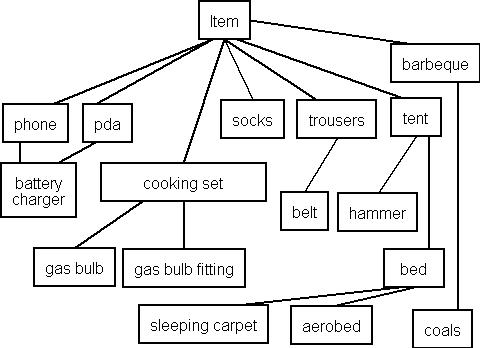
\includegraphics{subcomponents.jpg}
\end{center}
\caption{Required components}
\label{figuur:RequiredComponents}
\end{figure}


\paragraph{Required Functions}

\begin{itemize}
\item ...
\end{itemize}

\paragraph{Incompatible Components}

\begin{itemize}
\item Hotel guide <-> Tent
\end{itemize}

\paragraph{Alternative Components}

\begin{itemize}
\item Cooking contruction <-> Barbeque
\item Phone <-> PDA
\end{itemize}


\section*{Knowledge About Configuration}

We can only take a total of 10 kilograms in our backpack.
Also, the components have to fit in the packpack.
The arrangement model therefore specifies the dimensions of the bag. 
Components with any of their three dimensions longer than the largest dimension 
of the bag will be excluded beforehand.


\section*{Knowledge About Sharing}

Hmmm, volgens mij hoort er bij MCF1 geen sharing (zo te zien
op de slides). Ik kan ook niet zo veel bedenken qua sharing
bij deze opdracht...


\section*{Possible Scenario}

The following is part of a possible scenario of applying the
MCF1 technique.

\paragraph{Functional Requirements}

To go on a camping holiday, we need to arrange for the following
in our backpack: something to prepare food, a place to sleep.

\paragraph{Key Components}

From these functional requirements we pick our key components. For
the first one, something to prepare food, we can choose between a
barbeque and a cooking construction. However, our evaluation
function says we prefer eating cooked food over eating barbequed
food, so we choose the cooking construction.

For the second requirement, a place to sleep, we can choose between
a tent and a hotel guide. Of course, we prefer sleeping in a tent,
so we take the tent.

\paragraph{Required Components}

The cooking construction we choose requires a cooking pan to go
with it. So we add the cooking pan to our configuration. The tent
requires something to sleep on, which can be either an aerobed or
a sleeping carpet. (kies op basis van gewicht ofzo)

\paragraph{Arranging Components}

Now we have satisfied all functional requirements and dependencies,
we try to arrange the choosen components to form a configuration.

(kijk of gewicht goed is en of alles in de backpack past)


\end{document}
